\documentclass[12pt]{exam}
\usepackage[hon]{template-for-exam}
\usepackage{tikz,ifthen}
\footer{}{}{}
\header{}{}{}
\shadedsolutions
%\printanswers



\begin{document}

\def\mystrut{\protect\rule[-2.2ex]{0ex}{2.2ex}} 
\qformat{ \textbf{Task \#\thequestion}
  \ifthenelse{\equal{\thequestion}{\thequestiontitle}}
    {}
    {: \emph{\thequestiontitle}}
  \mystrut  \hfill}
\begin{questions}
  
\question
  
  Vectors $\vec{A}$ and $\vec{B}$ are shown below.

  \begin{parts}
    \part 
      Find the components of $\vec{A}$ and $\vec{B}$. {\sc Rotate Marker}
      %
      \begin{solution}
        \begin{align*}
          A_x &= \SI{ 9.21}{\meter\per\second} &
          A_y &= \SI{ 3.91}{\meter\per\second} \\
          B_x &= \SI{ 5.36}{\meter\per\second} &
          B_y &= \SI{-4.49}{\meter\per\second} 
        \end{align*}
      \end{solution}
    \part
      Sketch out what $\vec{R}=\vec{A}-2\vec{B}$ would look like. {\sc Rotate Marker}
      %
      \begin{solution}

        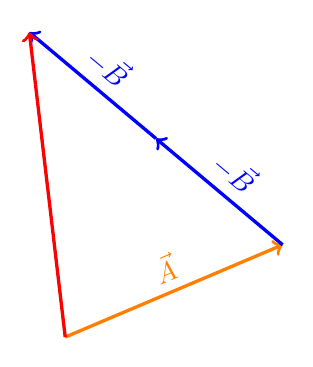
\begin{tikzpicture}[
          vector/.style={
            ->,
            very thick,
          }
        ]
        \def\unit{0.3}
          \draw[vector,orange] (0,0) -- 
            (23:10*\unit) coordinate (end A)
            node[midway,above,rotate=23] {$\vec{A}$};

          \draw[vector,blue] (end A) -- 
            ++(-40:-7*\unit) coordinate (end B)
            node[midway,above,rotate=-40] {$-\vec{B}$};

          \draw[vector,blue] (end B) -- 
            ++(-40:-7*\unit) coordinate (end C)
            node[midway,above,rotate=-40] {$-\vec{B}$};

          \draw[vector,red] (0,0) -- (end C);
        \end{tikzpicture}
      \end{solution}
    \part
      Calculate the magnitude and direction of $\vec{R}$

      \begin{solution}
        \begin{align*}
          R_x     &= \SI{-1.51}{\meter\per\second} &
          R_y     &= \SI{12.89}{\meter\per\second} \\
          \vec{R} &= \SI{12.98}{\meter\per\second} \text{\@ 83.3$^\circ$ N of W}
        \end{align*}
      \end{solution}
  \end{parts}

  \vspace{1em}

  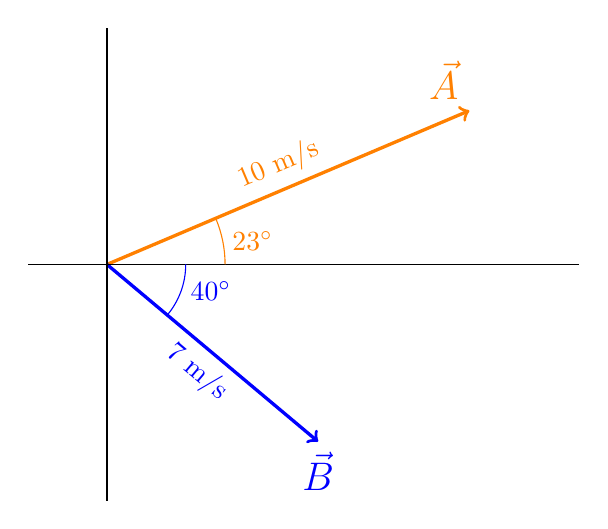
\begin{tikzpicture}[
    vector/.style={
      ->,
      very thick,
    }
  ]
    \def\unit{0.5}
    

    \draw[vector,orange] (0,0) -- (23:10*\unit) 
      node[anchor=south east] {\Large $\vec{A}$} 
      node[midway,above,rotate=23] {10 m/s};
    \draw[vector,blue] (0,0) -- (-40:7*\unit)
      node[anchor=north] {\Large $\vec{B}$}
      node[midway,below,rotate=-40] {7 m/s};
    \draw (0,3) -- (0,-3);
    \draw (-1,0) -- (6,0);

    \draw[orange] (1.5,0) arc (0:23:1.5) 
      node[midway,right] {$23^\circ$};
    \draw[blue] (1,0) arc (0:-40:1) 
      node[midway,right] {$40^\circ$};



  \end{tikzpicture}

  \vs \hrule \vs

  \question
    The summit of a mountain, 2450 m above base camp, is measured on a map to be 4580 m horizontally from the camp in a direction 38.4$^\circ$ west of north.
    

    \begin{parts}
      \part
        Find the $x$-, $y$-, and $z$- components of the displacement vector from camp to summit.  (Use $+x$ as east, $+y$ as north and $+z$ as up.) {\sc Rotate Marker}
        %
        \begin{solution}
          \begin{align*}
            D_x &= \SI{-2844.9}{\meter} &
            D_y &= \SI{ 3589.3}{\meter} &
            D_z &= \SI{ 2450  }{\meter} 
          \end{align*}
        \end{solution}
      \part
        Find the magnitude of the displacement vector.
        %
        \begin{solution}
          \begin{align*}
            D &= \SI{5194.1}{\meter} &
          \end{align*}
        \end{solution}
    \end{parts}

    \vs \hrule \vs

  \question
    You are at a location 3600 meters at a direction 35$^\circ$ south of east from a watchtower.  Your endpoint is 2300 meters due west of the watchtower.  How far and in what direction should you travel to get to your endpoint?
    %
    \begin{solution}

      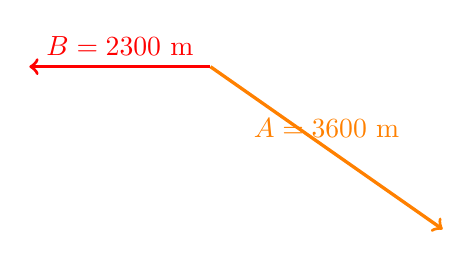
\begin{tikzpicture}[
        vector/.style={
          ->,
          very thick,
        }
      ]
        \def\unit{0.1}
        
    
        \draw[vector,orange] (0,0) -- (-35:36*\unit) 
          node[above, midway] {$A = 3600$ m};
        \draw[vector,red] (0,0) -- (-180:23*\unit)
          node[above, midway] {$B = 2300$ m};
    
      \end{tikzpicture}

      \begin{align*}
        \vec{A} + \vec{R} &= \vec{B} \\
        \vec{R}           &= \vec{B} - \vec{A}
      \end{align*}

      \begin{align*}
        A_x &= 2948.9 &
        A_y &= -2064.9\\
        B_x &= -2300 &
        B_y &= 0 \\\\
        R_x &= -5248.9 &
        R_y &= 2064.9 \\
        \vec{R} &= 5640.5~\text{m @ 21.5 $^\circ$ W of N}
      \end{align*}
    \end{solution}


\end{questions}




\end{document}